\documentclass[portrait,a0paper,fontscale=0.35]{baposter}

\usepackage{calc}
\usepackage{graphicx}
\usepackage{amsmath}
\usepackage{amssymb}
\usepackage{relsize}
\usepackage{multicol}
\usepackage{multirow}
\usepackage{rotating}
\usepackage{bm}
\usepackage{url}

\usepackage{graphicx}
\usepackage{multicol}

\begin{document}

\begin{poster}{
  grid=false,
  columns=4,
  colspacing=1em,
  bgColorOne=white,
  bgColorTwo=white,
  borderColor=blue,
  headerColorOne=black,
  headerColorTwo=blue,
  headerFontColor=white,
  boxColorOne=white,
  boxColorTwo=blue,
  textborder=roundedleft,
  eyecatcher=true,
  headerborder=closed,
  headerheight=0.1\textheight,
  headershape=roundedright,
  headershade=shadelr,
  headerfont=\Large\bf\textsc,
  textfont={\setlength{\parindent}{1.5em}},
  boxshade=plain,
  background=plain,
  linewidth=2pt
  }
  {
  }
  {\bf\textsc{Analysis of the Biomodels Database}\vspace{0.5em}}
  {Unknown Author}
  {
  }
  
 \headerbox{Biomodels Database}{name=biomodelsdatabase,column=0,row=0}{
 Biomodels Database is an online resource for storing and serving quantative models of biomedical  interest. The database is composed of two branches, of these is the curated branch, which is the focus of this project. There are currently 421 models in the curated branch. These models have been described in peer reviewed sceintific literature.
 
 One of the languages used by modellers submitting to the biomodels datbase is SBML. The models can also be downloaded from the database in SBML format.
 
 }
  
  \headerbox{R}{name=r, column=1,row=0}{
  R is a computer package that is widely used for statistical software
development and data analysis. The system
provides a wide variety of statistical and graphical techniques.
 
 R is highly extensible through the use of user-submitted libraries for
specific functions or specific areas of study. An example of this is the package rsbml, which was used in order to read models into R and extract information from the models.
 
 A particular strength of R is its graphical facilities, which produce quality graphs that can include
mathematical symbols.
  }
 
 \headerbox{Species and Reactions}{name=specsnreacts,column=2,row=0,span=2}{
 \begin{multicols}{2}
 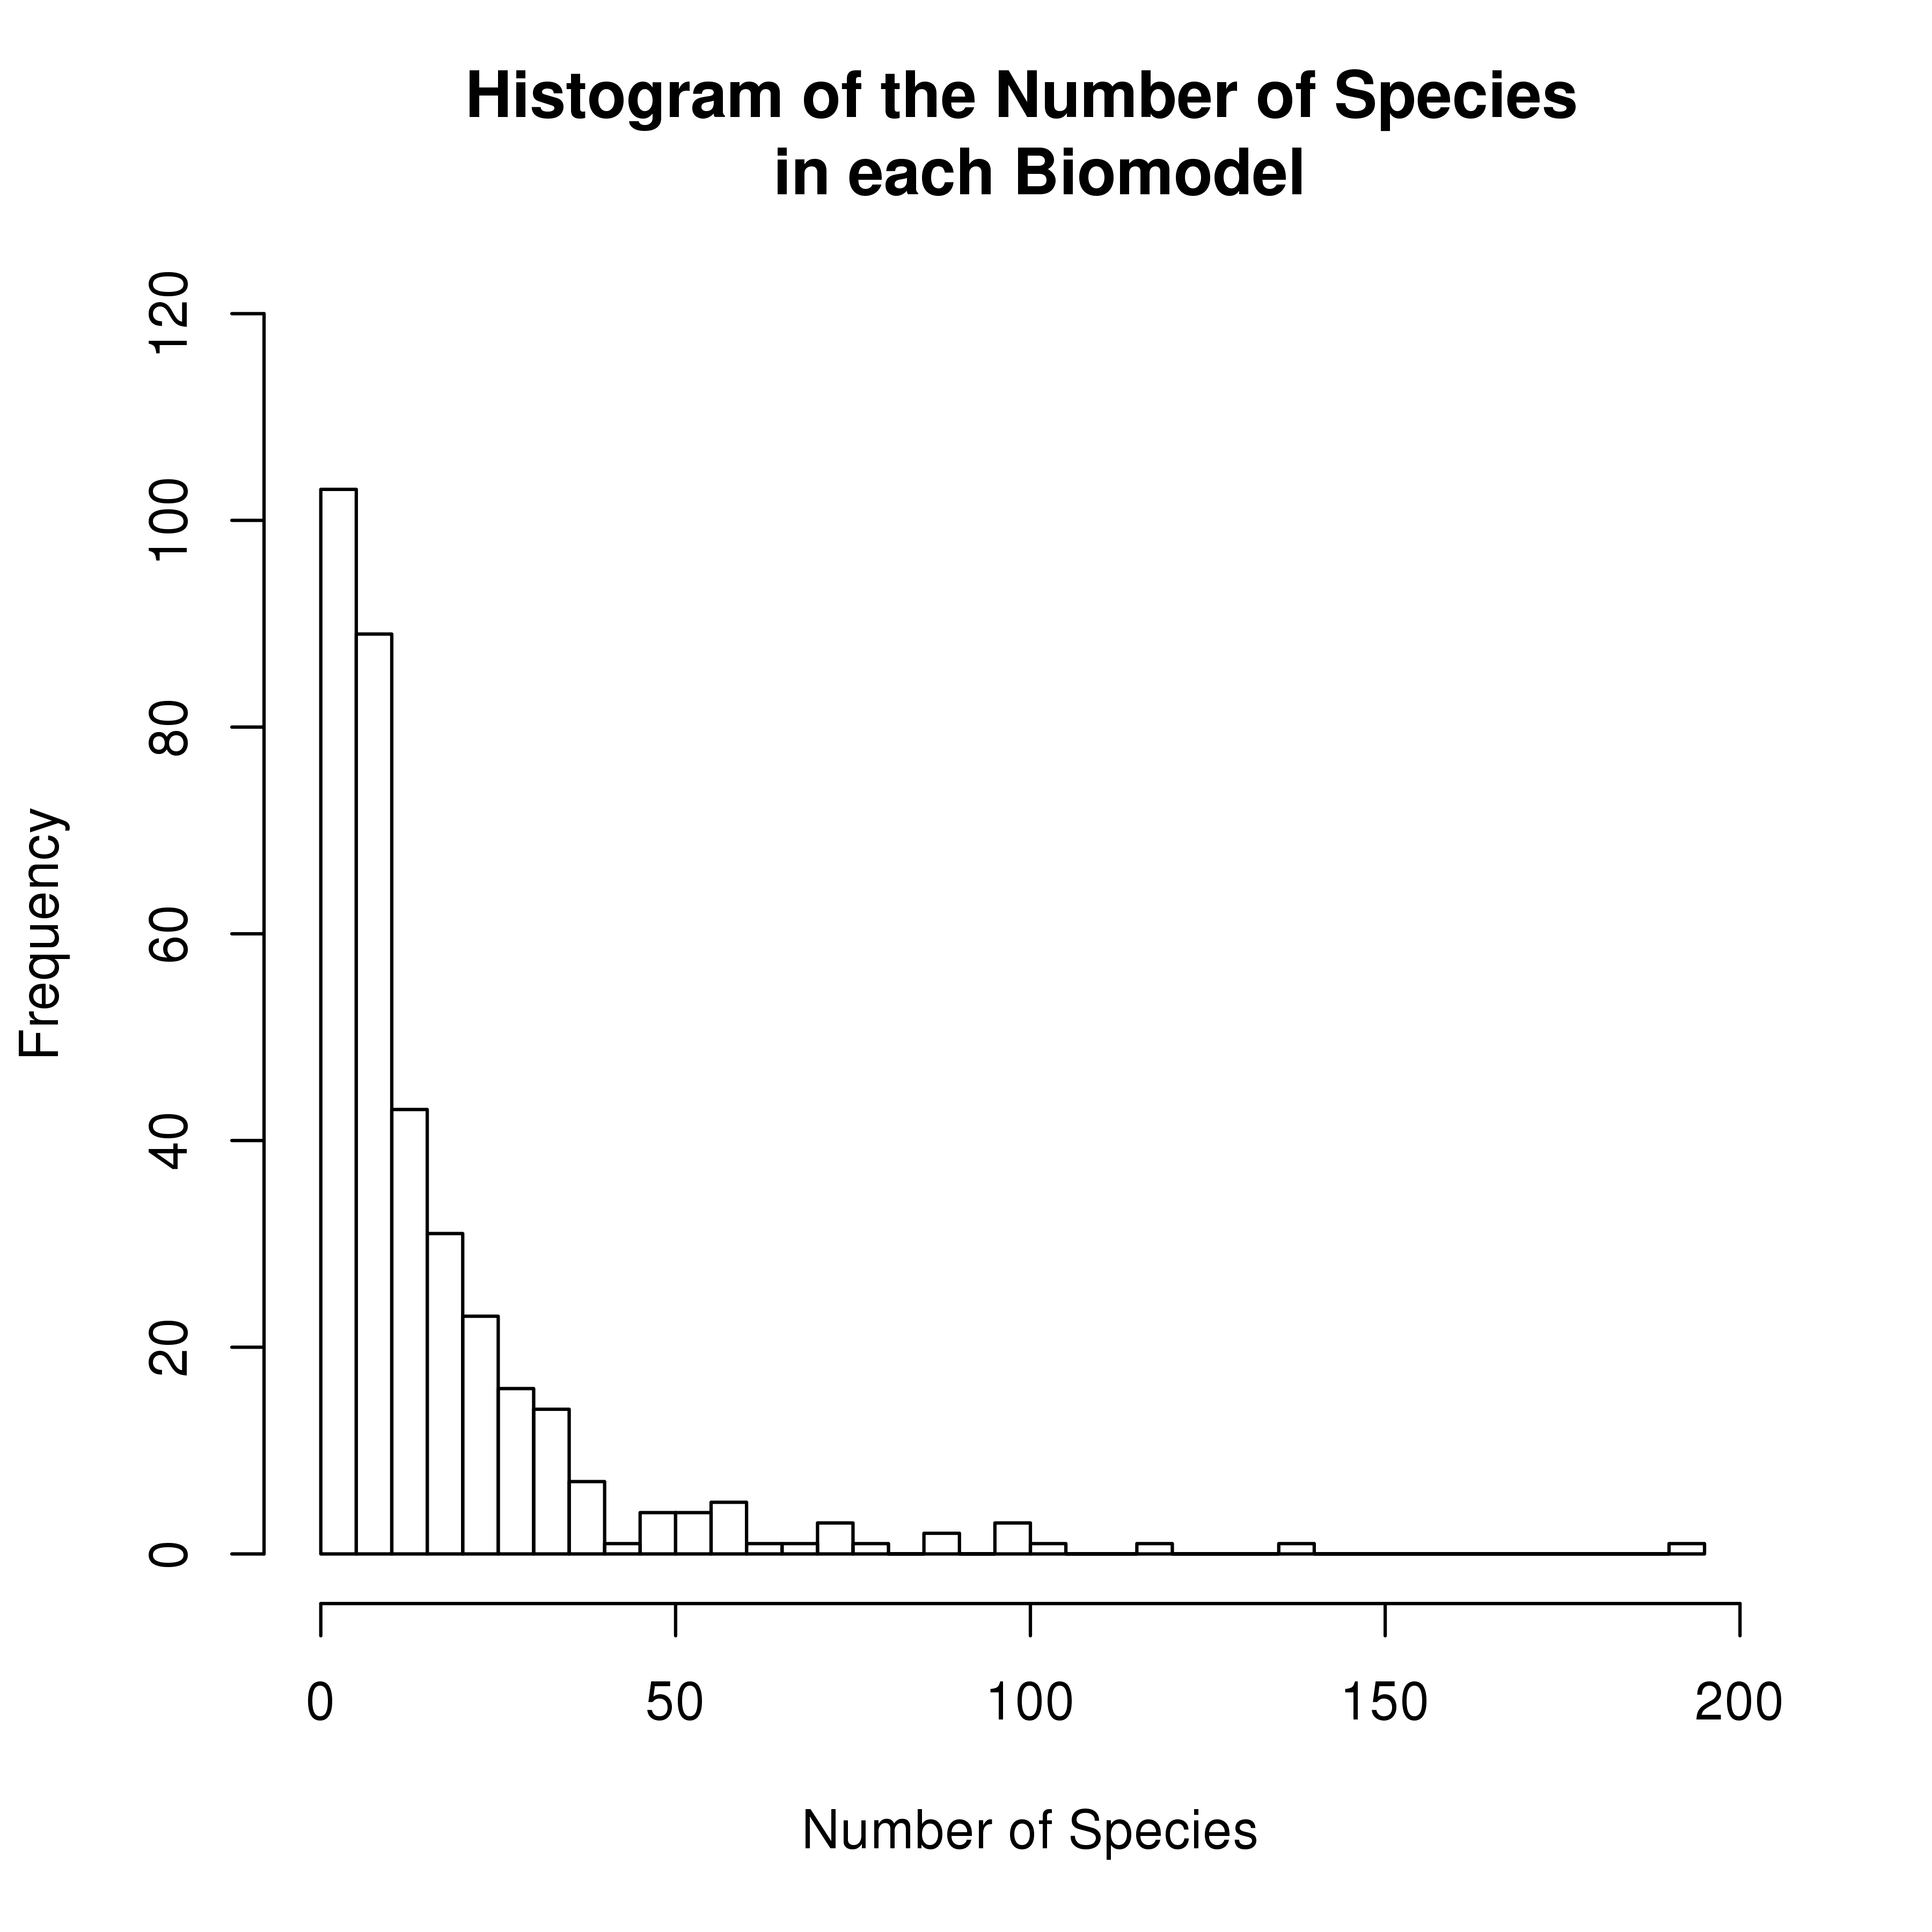
\includegraphics[trim= 1.5mm 5mm 5mm 5mm, clip, scale=0.4]{Poster-images/SpeciesHistogram.png}
 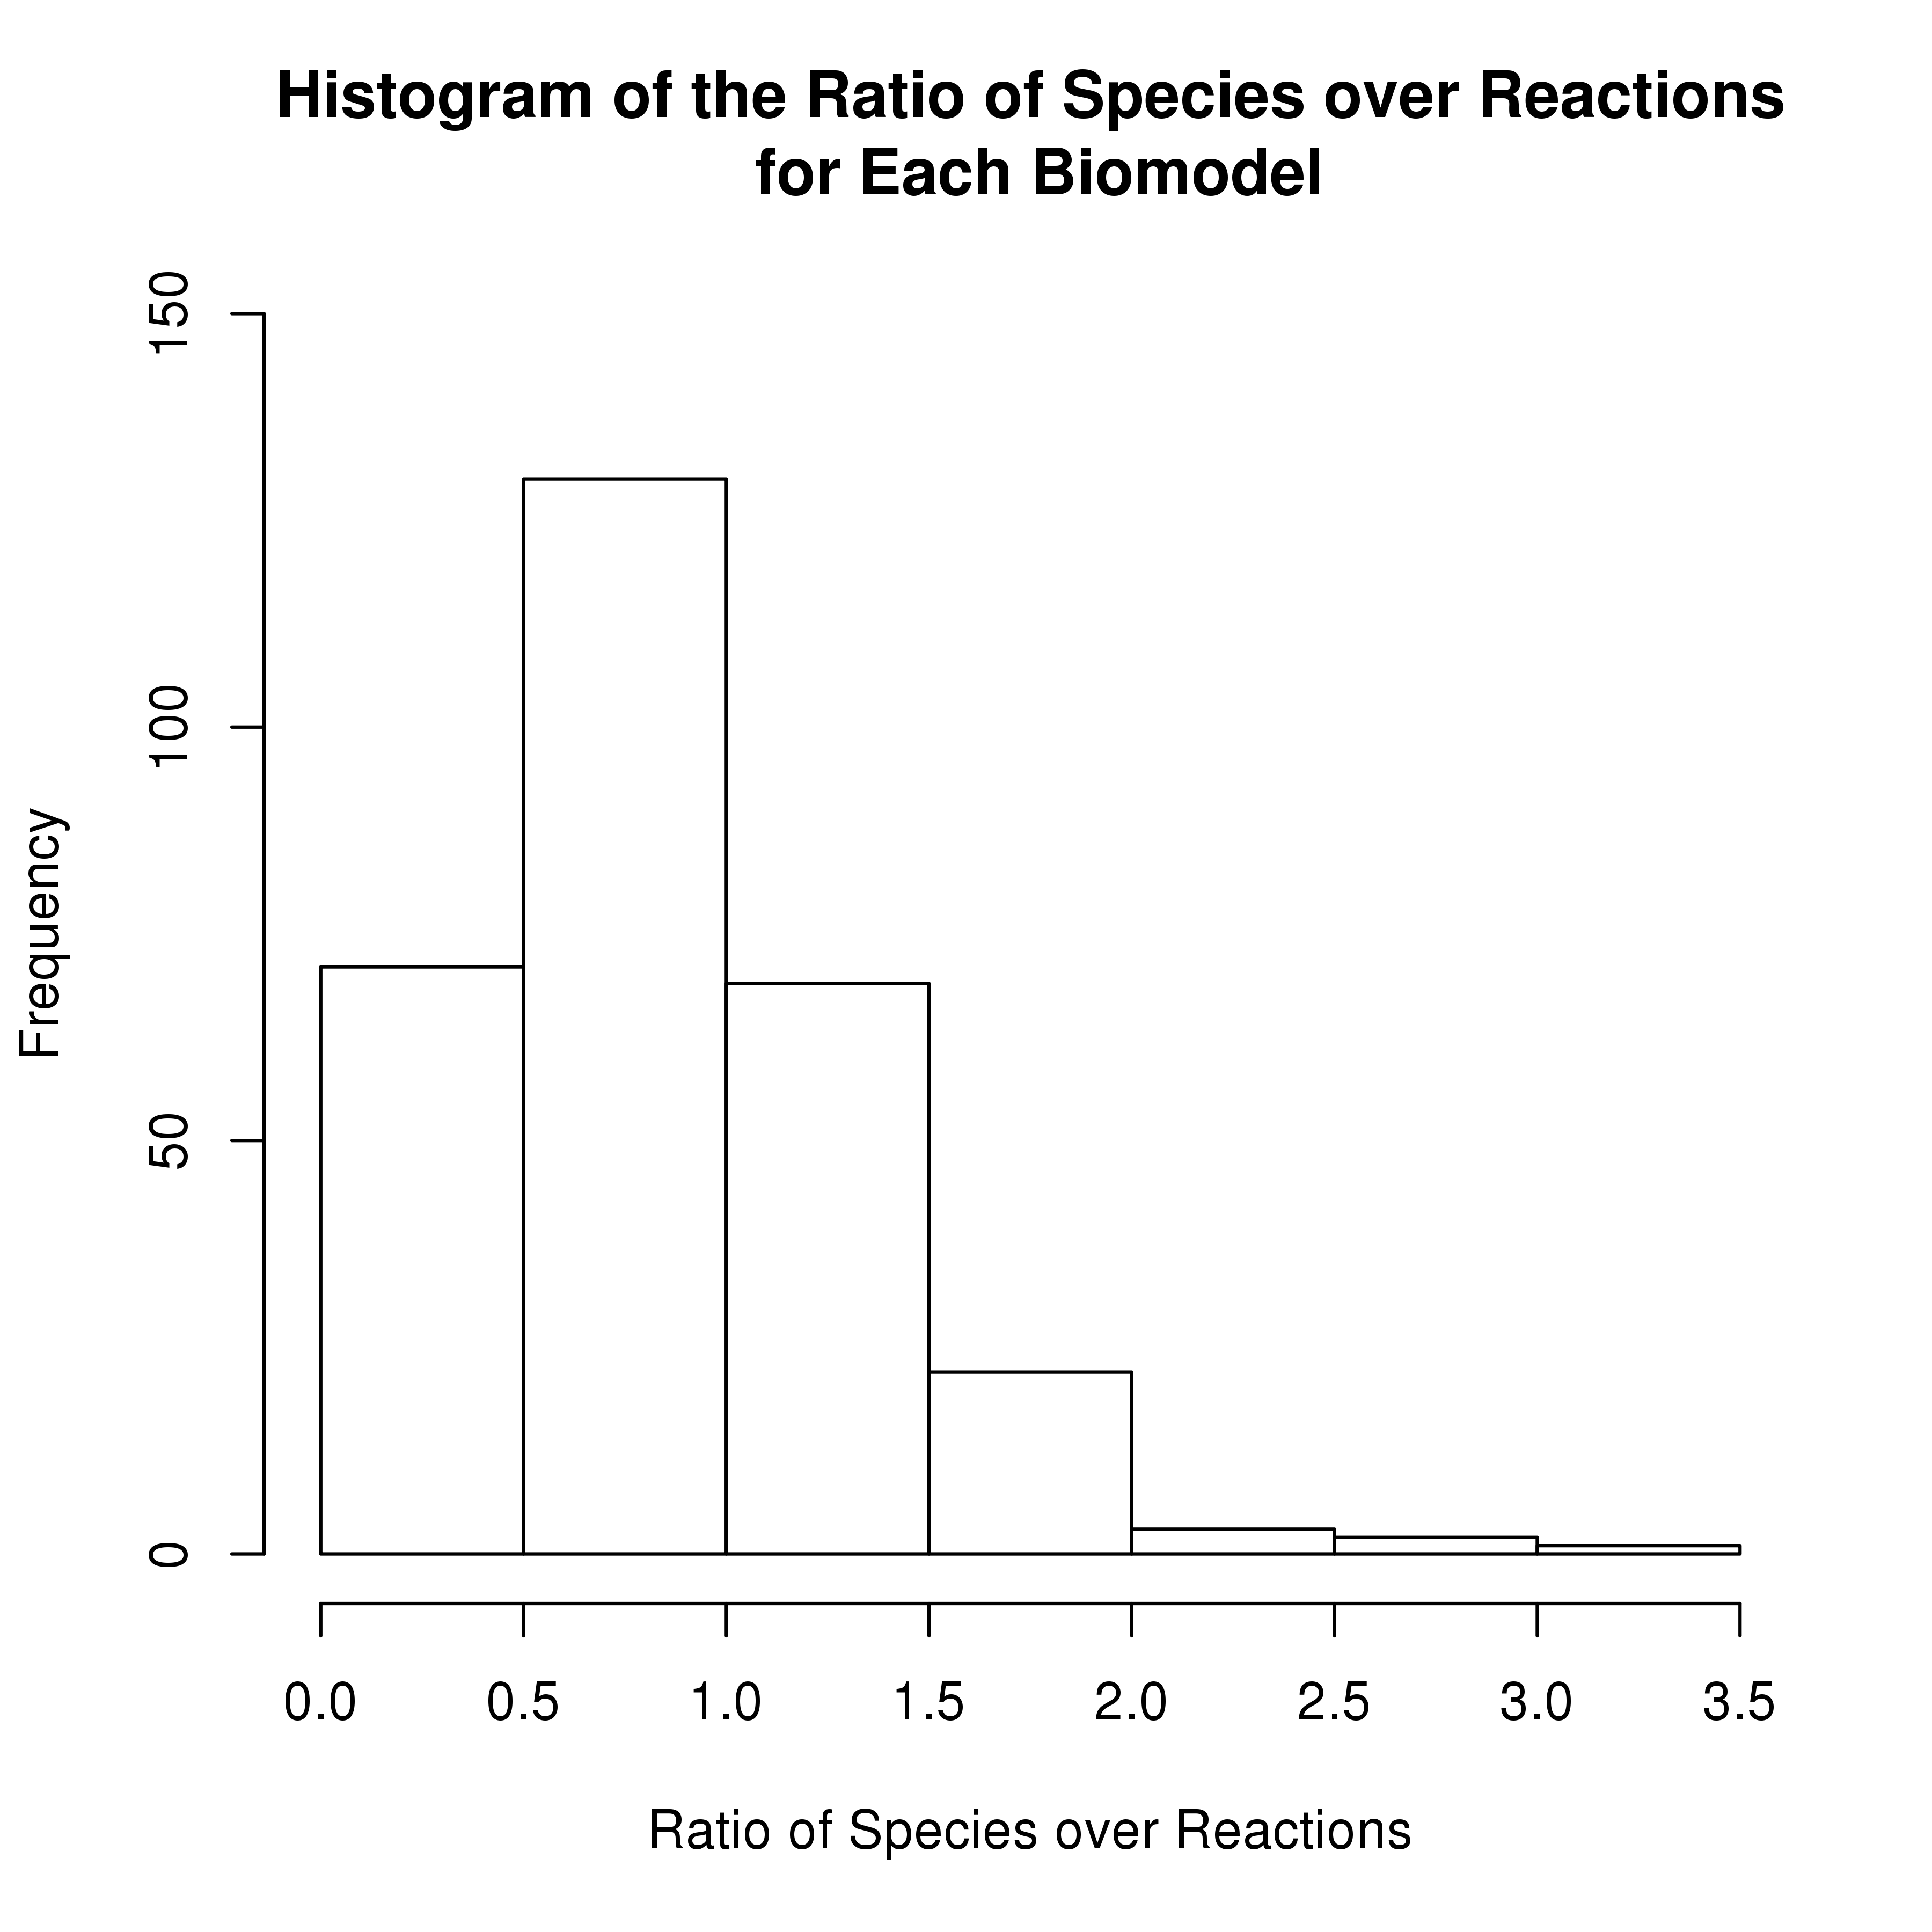
\includegraphics[trim= 1.5mm 5mm 5mm 5mm, clip, scale=0.4]{Poster-images/SpeciesOverReactions.png}
 
 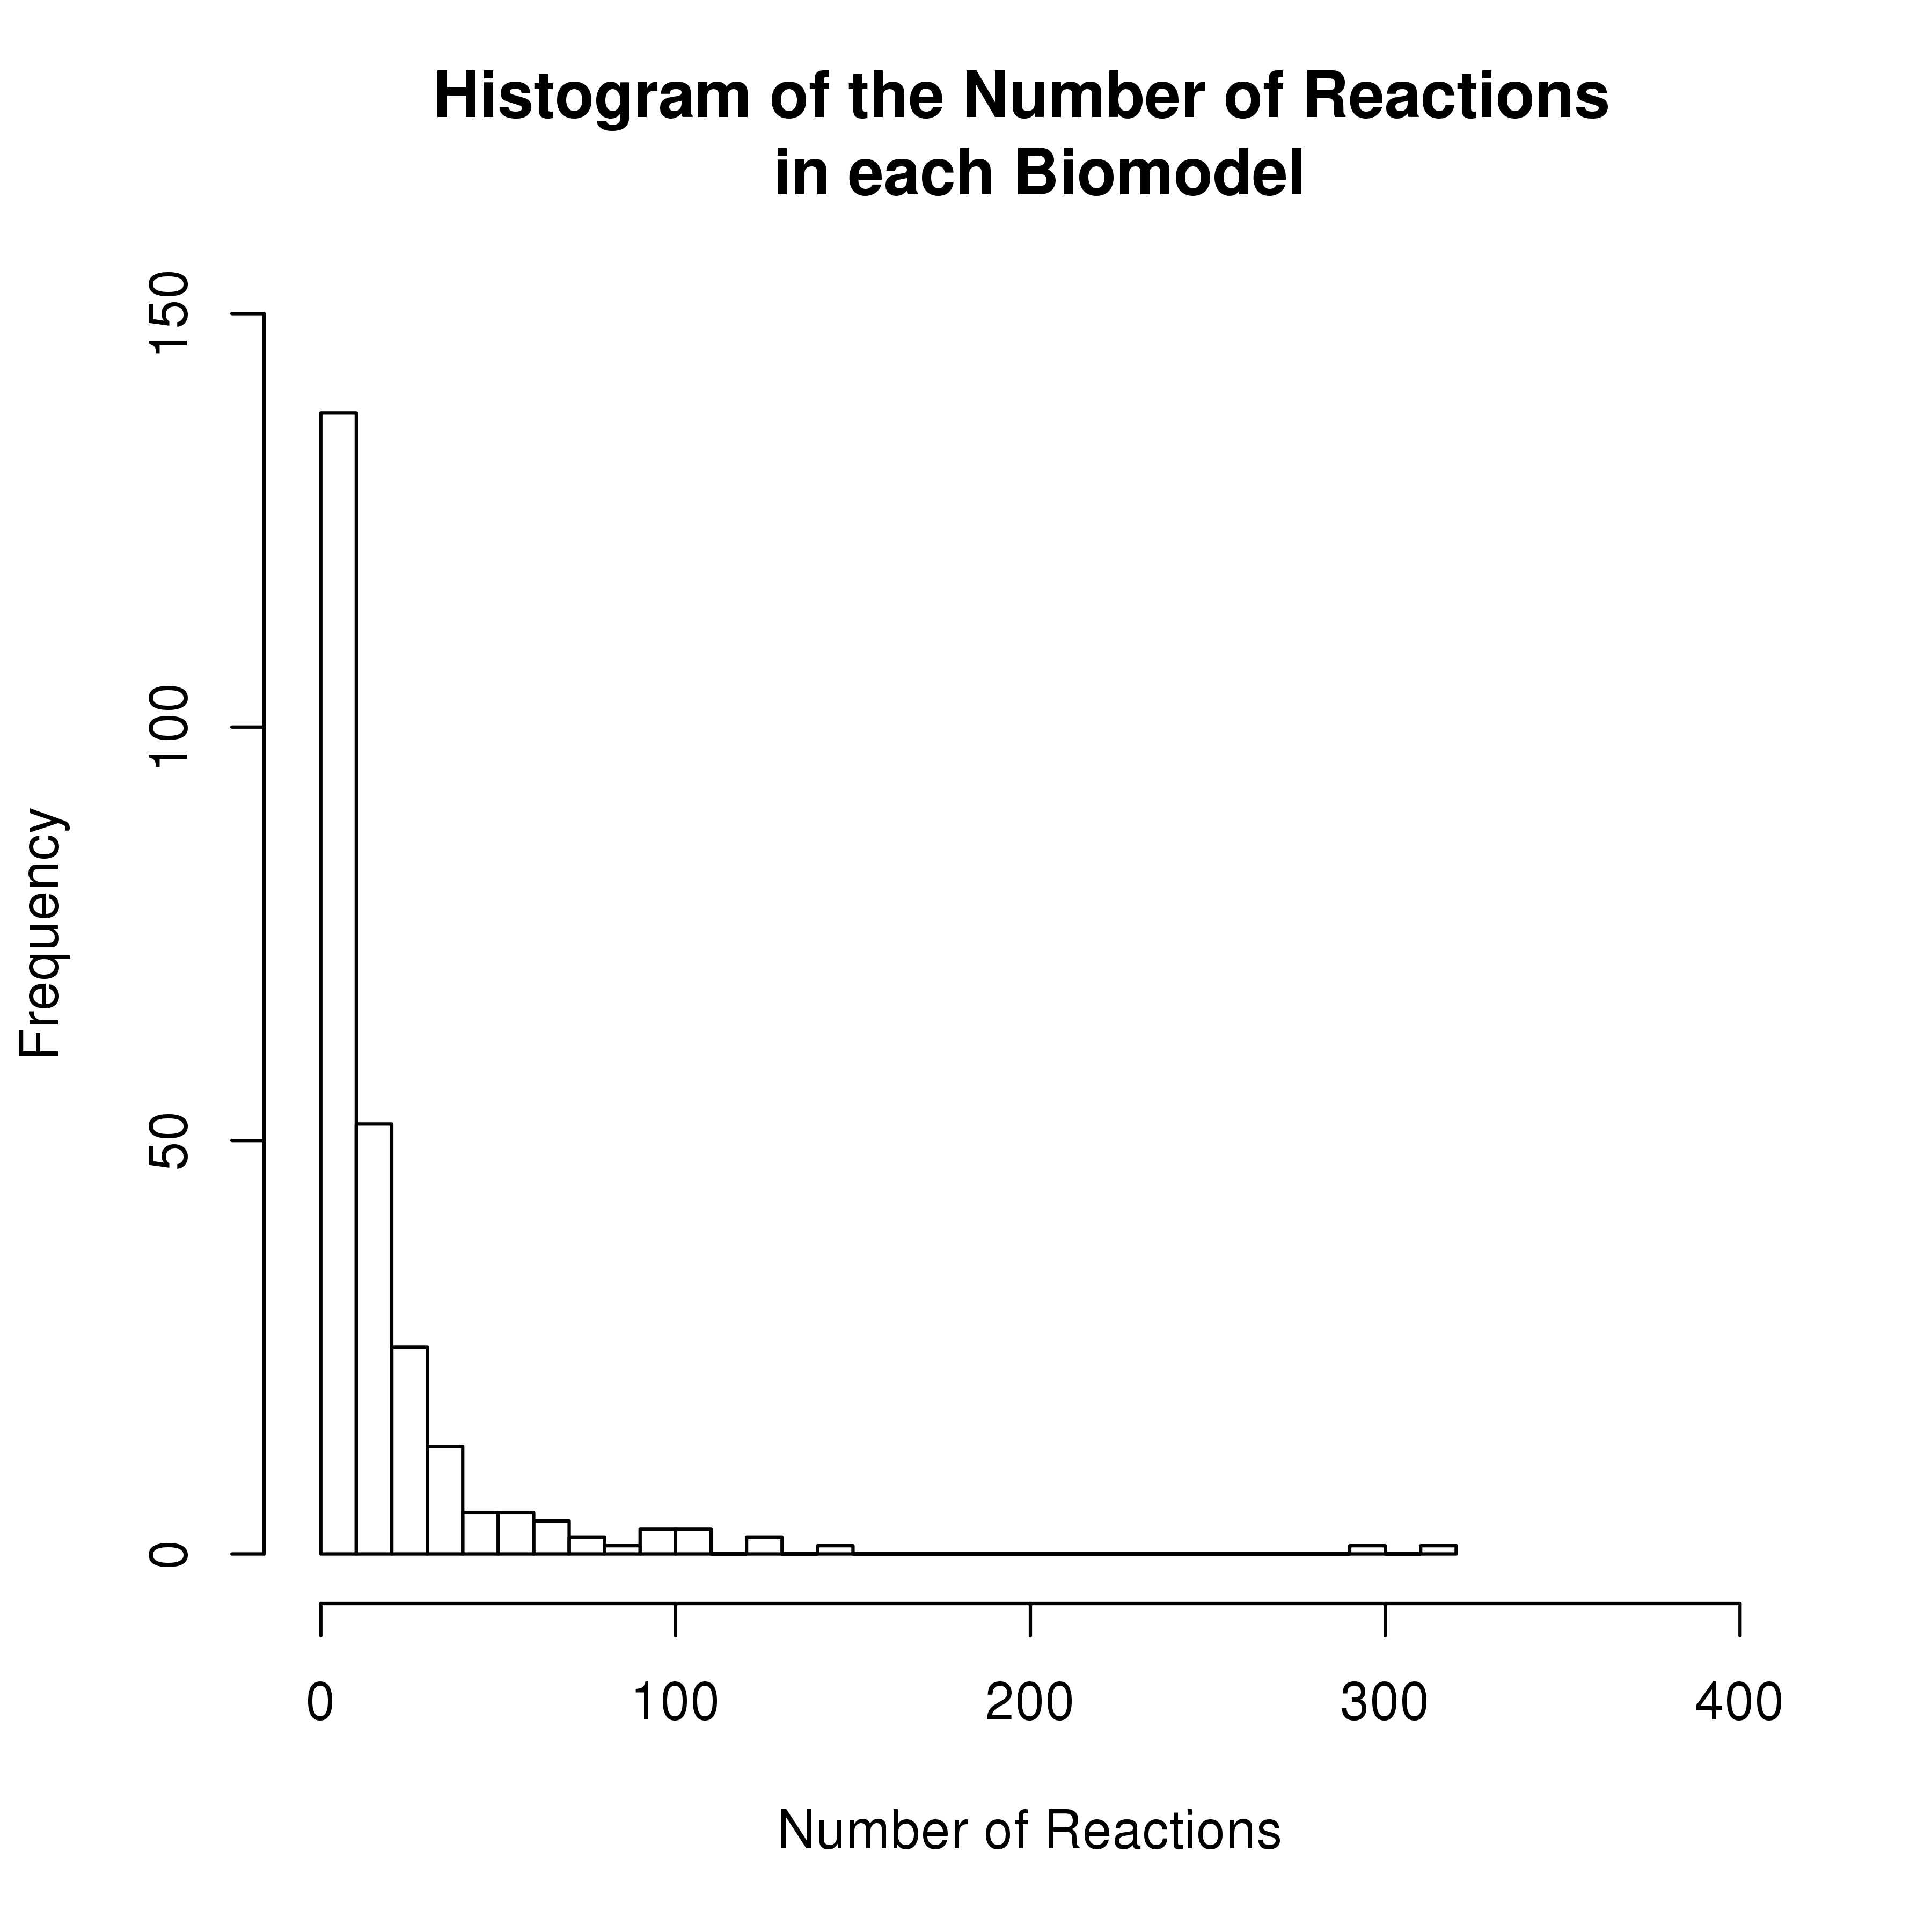
\includegraphics[trim= 1.5mm 5mm 5mm 5mm, clip, scale=0.4]{Poster-images/ReactionsHistogram.png} 
 The top left grpah is the histogram of the number of species in each biomodel. The majority of models have less than 20 species.
  This suggests that the majority of models have a small number of species. The histogram of reactions, the top right graph, displays a similar pattern, suggesting that the majority of models have a small number of species.
  The graph to the left is a histogram of the ratio of species to reactants in each biomodel. The most frequent range is range of values is 0.5-1.0 with the majority of models having ratios less than 2. This suggest that the ratio of species to reactions is not particularly high for most models.
 \end{multicols}
 }
 
 
 \headerbox{References}{name=sboterms,column=0,above=bottom}{
 
 }
 
 \headerbox{Conlcusion}{name=conclusion,column=1,above=bottom}{
 
 }
 
 \headerbox{More Pretty Pictures}{name=moreprettypics,column=2,span=2,above=bottom}{
 \begin{multicols}{2}
 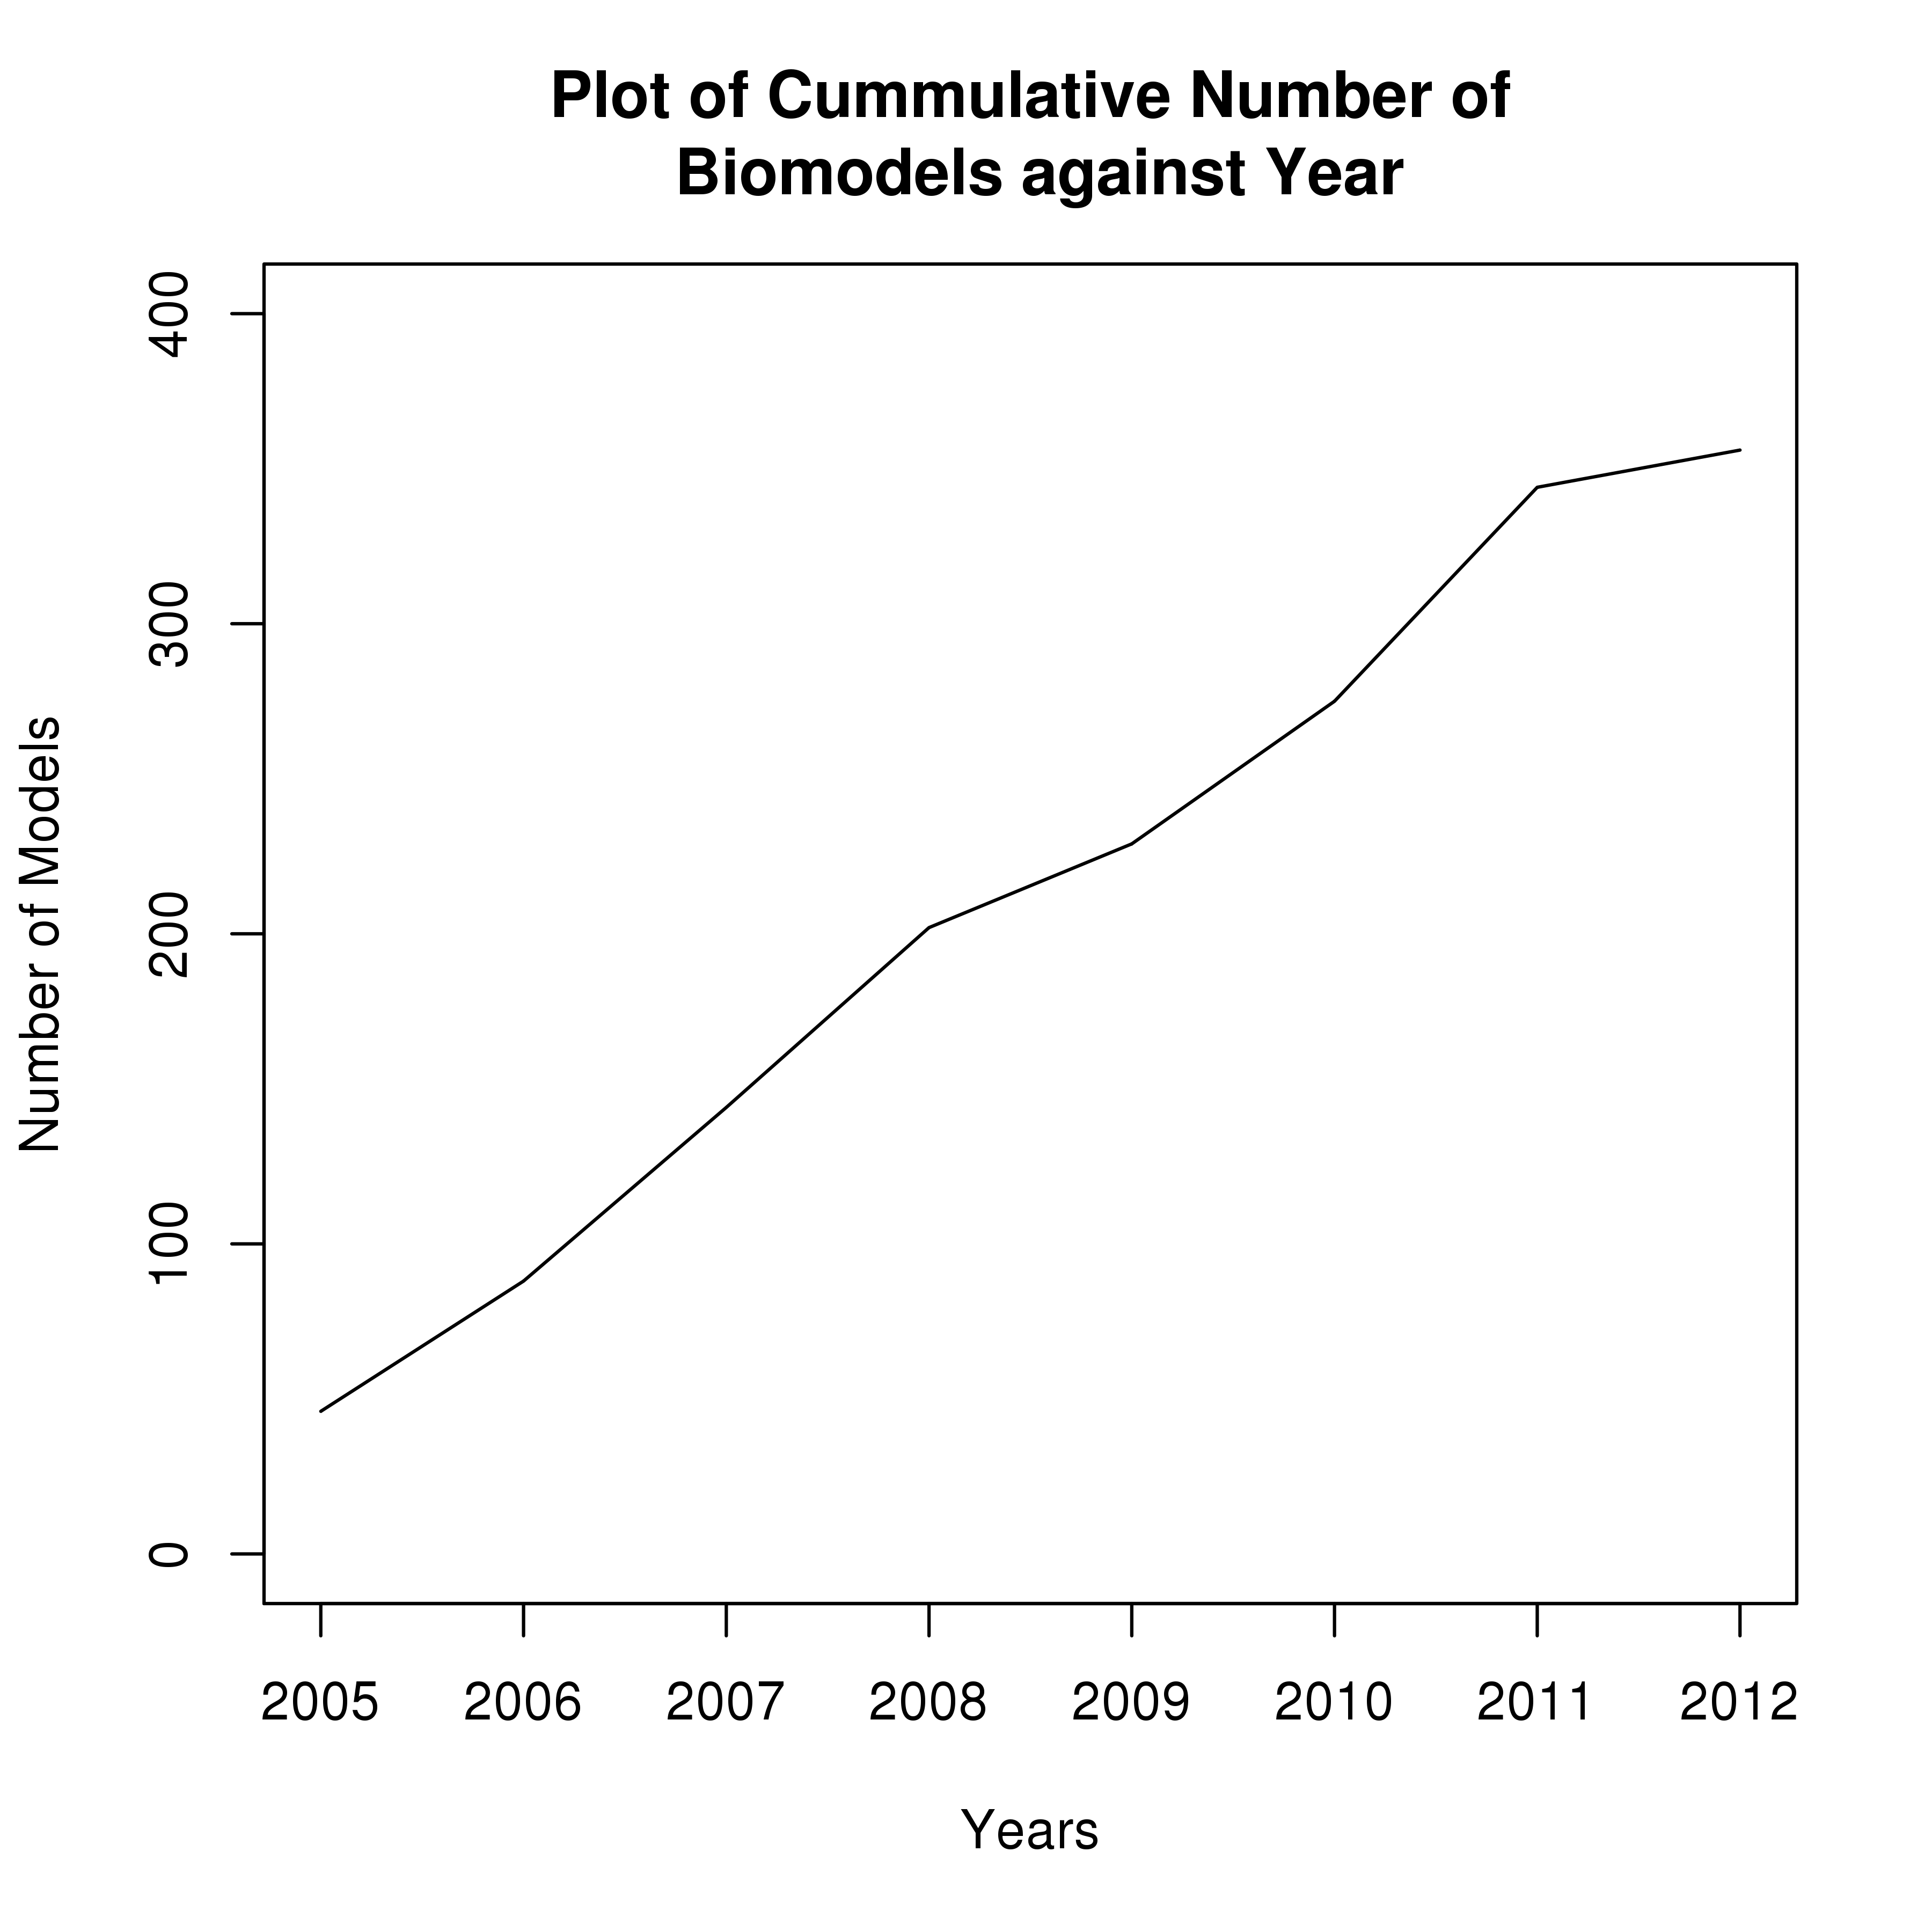
\includegraphics[trim= 1.5mm 5mm 5mm 4.5mm, clip, scale=0.4]{Poster-images/CummulativeModelsPlot.png}
 The above graphs shows how the number of biomodels in the curated branch of the database has varied over time, since  the first models were submitted. The increase in the number of models appears to be closer to expoential, suggesting that the rate at which models are added to the databse per year is increasing over time.
 The small increase in the number of models in the curated branch in 2012 is expected since the archive used in the project was the July 2012 archive.
 
 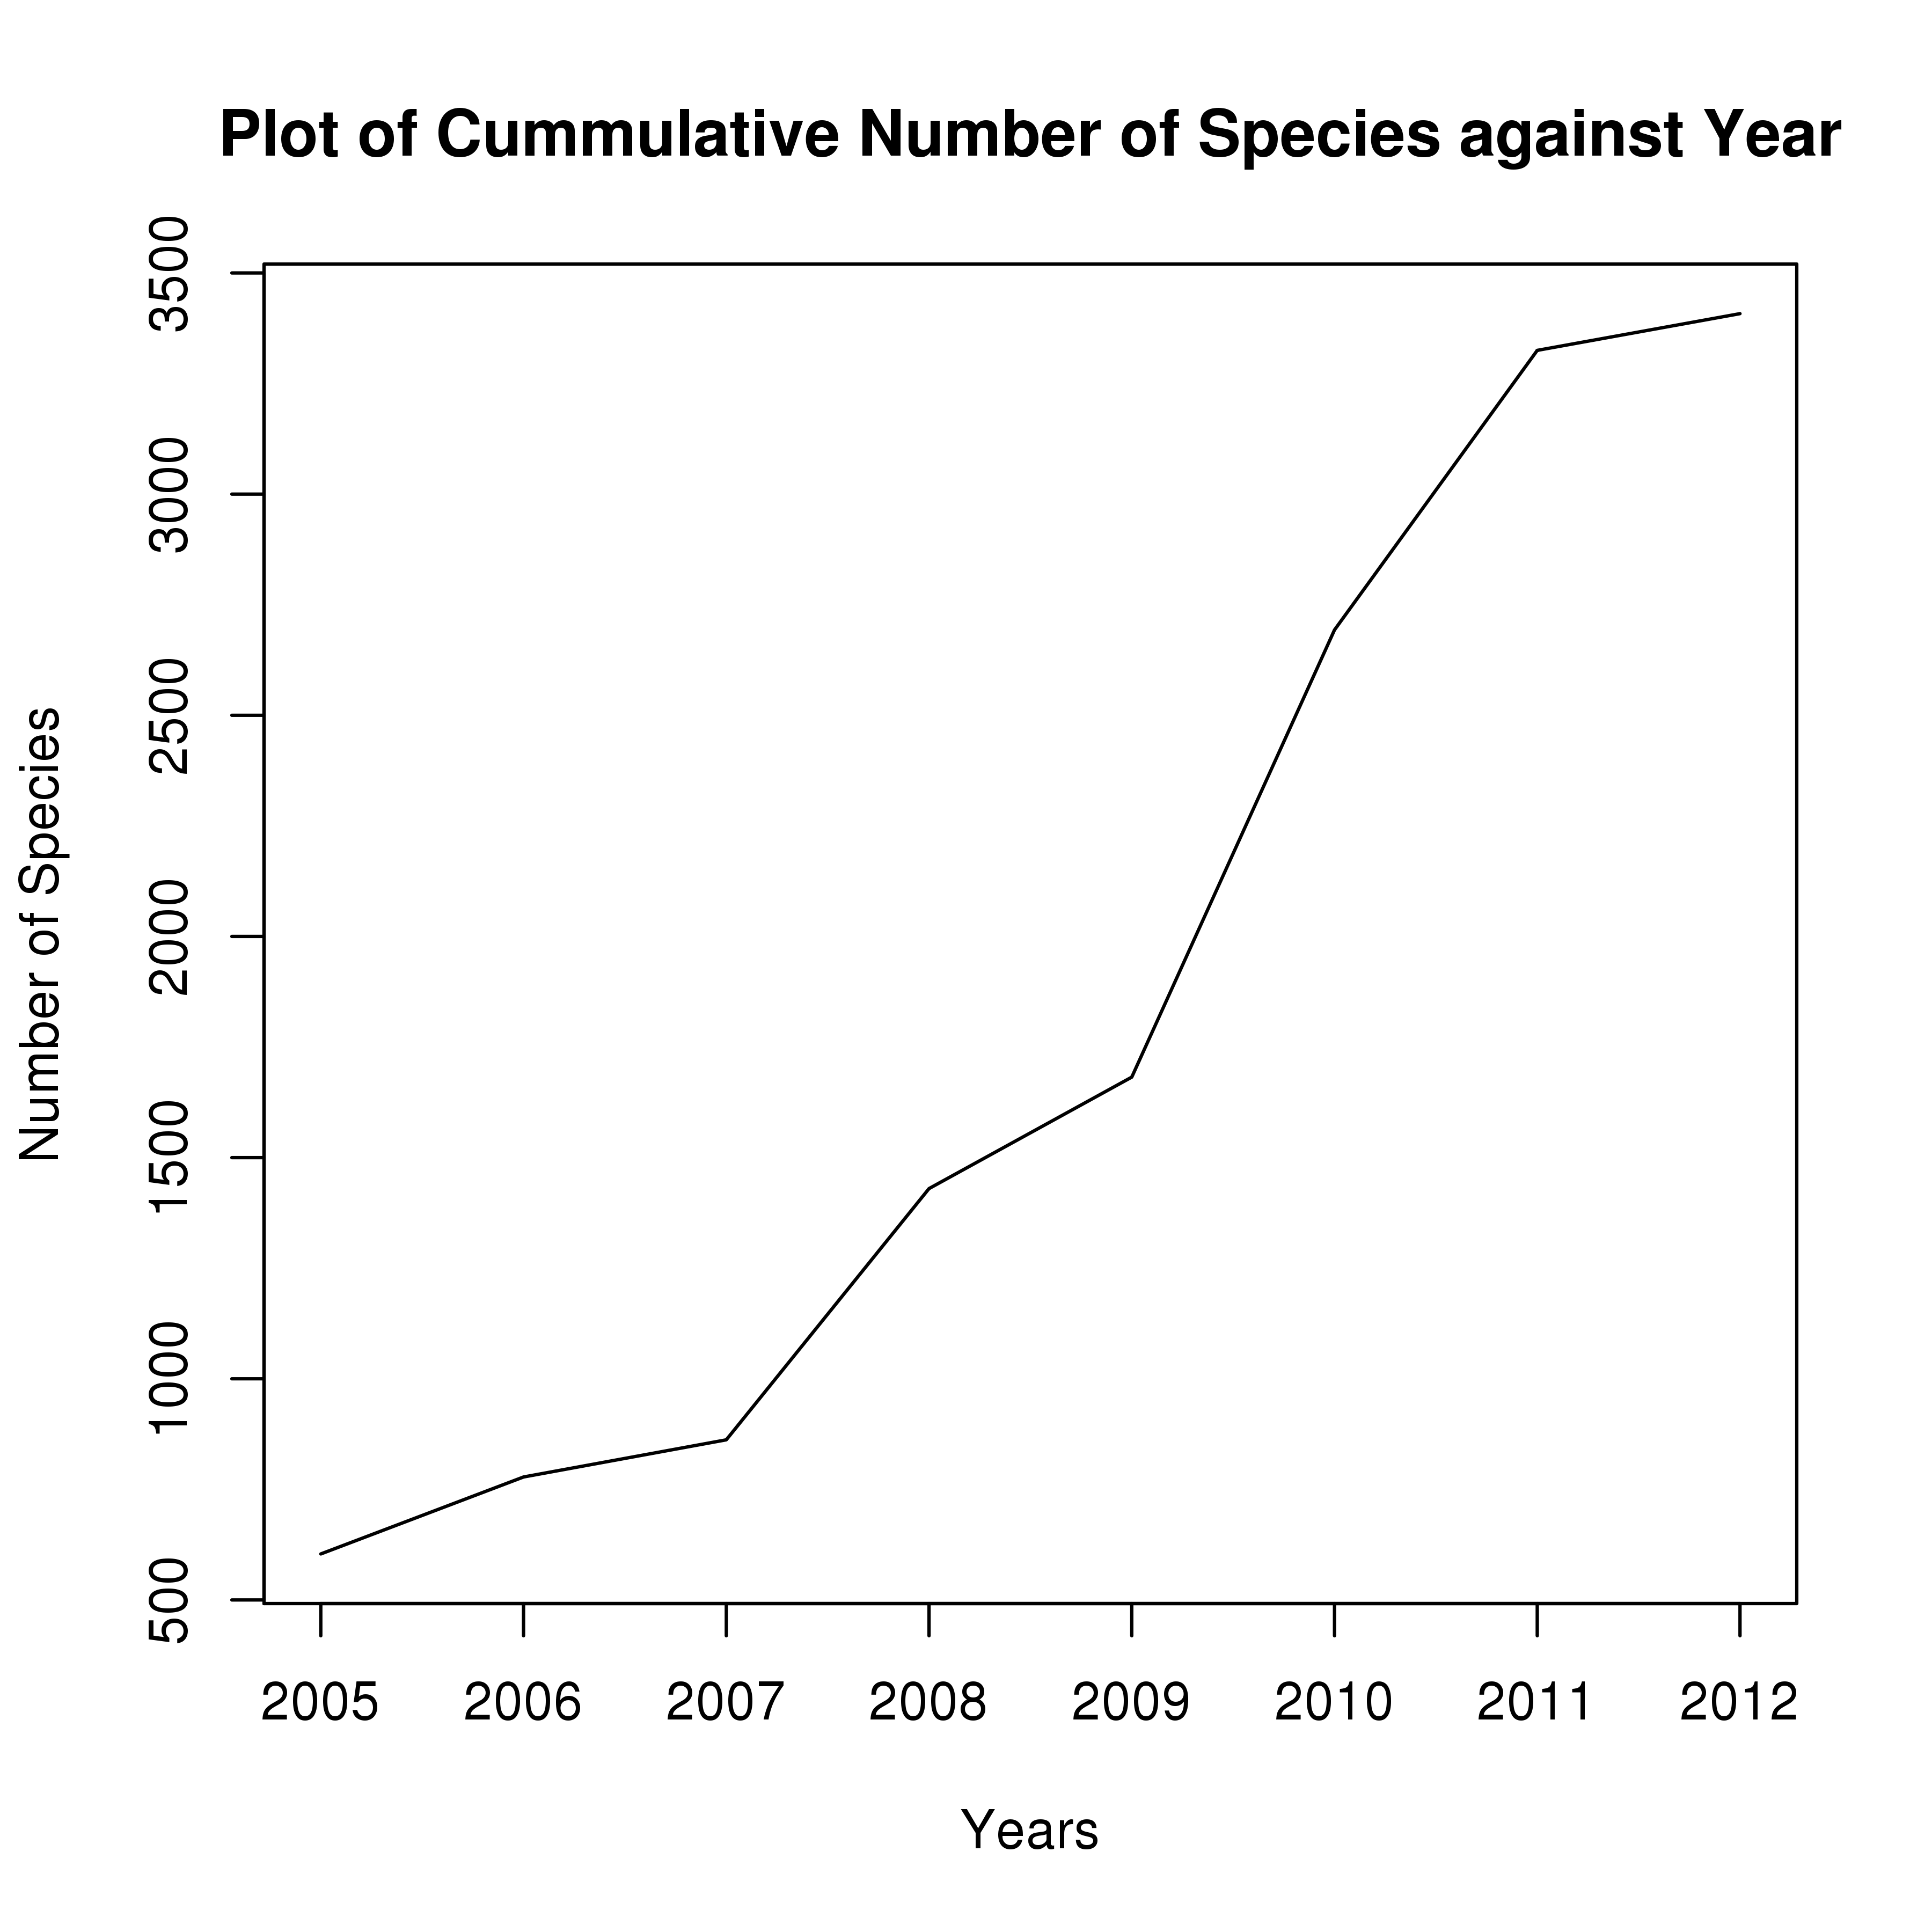
\includegraphics[trim= 1.5mm 5mm 5mm 4.5mm, clip, scale=0.4]{Poster-images/CummulativeSpeciesPlot.png}
 The above graphs shows how the numebr of species in the curated branch of the database has varied over time, since  the first models were submitted in 2005. As shown in the graph, the increse in the number of species is slightly more random than for the number of models. The only pattern is that a large increase in one year precedes a smaller increase in the next year.
 The small increase in the number of species in the curated branch in 2012 is expected, for the same reasons as for the number of models added in 2012.
 \end{multicols}
 }
 
 \headerbox{SBML}{name=sbml,column=0,span=2,below=r}{
 Systems Biology Markup Language (SBML) is an eXtensible Markup Language (XML) encoding of the reaction list, together with additional information required for quantitative modelling and simulation.
  
  SBML is used to represent biochemical networks in a way that is convinient for a computer to generate and parse. This allows the models to be communicated between disparate modelling and simulation tools.
  
  Whilst SBML is a good format to parse and generate, it is very difficult for humans to read and write. In order to extract infomation from the models during the project, the SBML files were first read into R and transformed into objects that could be worked with in R.
 }
 
 \headerbox{Terms}{name=terms,column=0,span=2,below=sbml}{
 \begin{multicols}{2}
 Consider we have a chemical called X. Let there be a model which describes how the amount of X varies with time where the rate of change of the amount of X is decribed by the following equation:\\
 
 $\frac{dX(t)}{dt} = \mu X(t) + \alpha$
 
 Where the amount of X is altered by the following processes:
 
 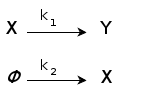
\includegraphics[scale=0.5]{Poster-images/TermDiagram.png}
 
 \begin{itemize}
 \item The entities X, Y and Z are species. Normally, species are chemicals such as ions or molecules but can also be biological entities such as protein binding sites.
 
 \vspace{1cm}
 
 \item The processes which alter the amount of X are called reactions. Reactions are the processes by which the amounts of the species in a model changes. The most common type involves a set of chemicals (reractants) being transfromed to another set of chemcials (products).
 
 \item $\mu$ and $\alpha$ are parameters. Parameters are the numbers which desrcibe the rate laws of reactions, this also describes how a species varies over time. Parameters can be constant or variable.
 
 \end{itemize}
 \end{multicols}
 }
 
  \headerbox{Connections}{name=connections,column=0,below=terms}{
 In this project, a species is defined as having a 'connection' in a particular reaction if the sepcies occurs in that reaction.\\
 
 Consider the following set of reactions:
 
 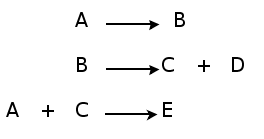
\includegraphics[scale=0.5]{Poster-images/connectiondrawing.png}
 
 Since A appears twice as a reactant, it has 2 connections. Since B appears as a product oncce and a reactnat once, it has two connections in total (one reactant and one product). D appears as product once and so only has one connection.\\
 
 The average number of connections per species in the database is 5.334 (to 3 decimal places). 
 }
 
 \headerbox{SBO Terms}{name=sboterms,column=1,below=terms}{
 
 }
 
 \headerbox{Parameters}{name=paras,column=2,span=2,below=specsnreacts}{
 \begin{multicols}{2}
 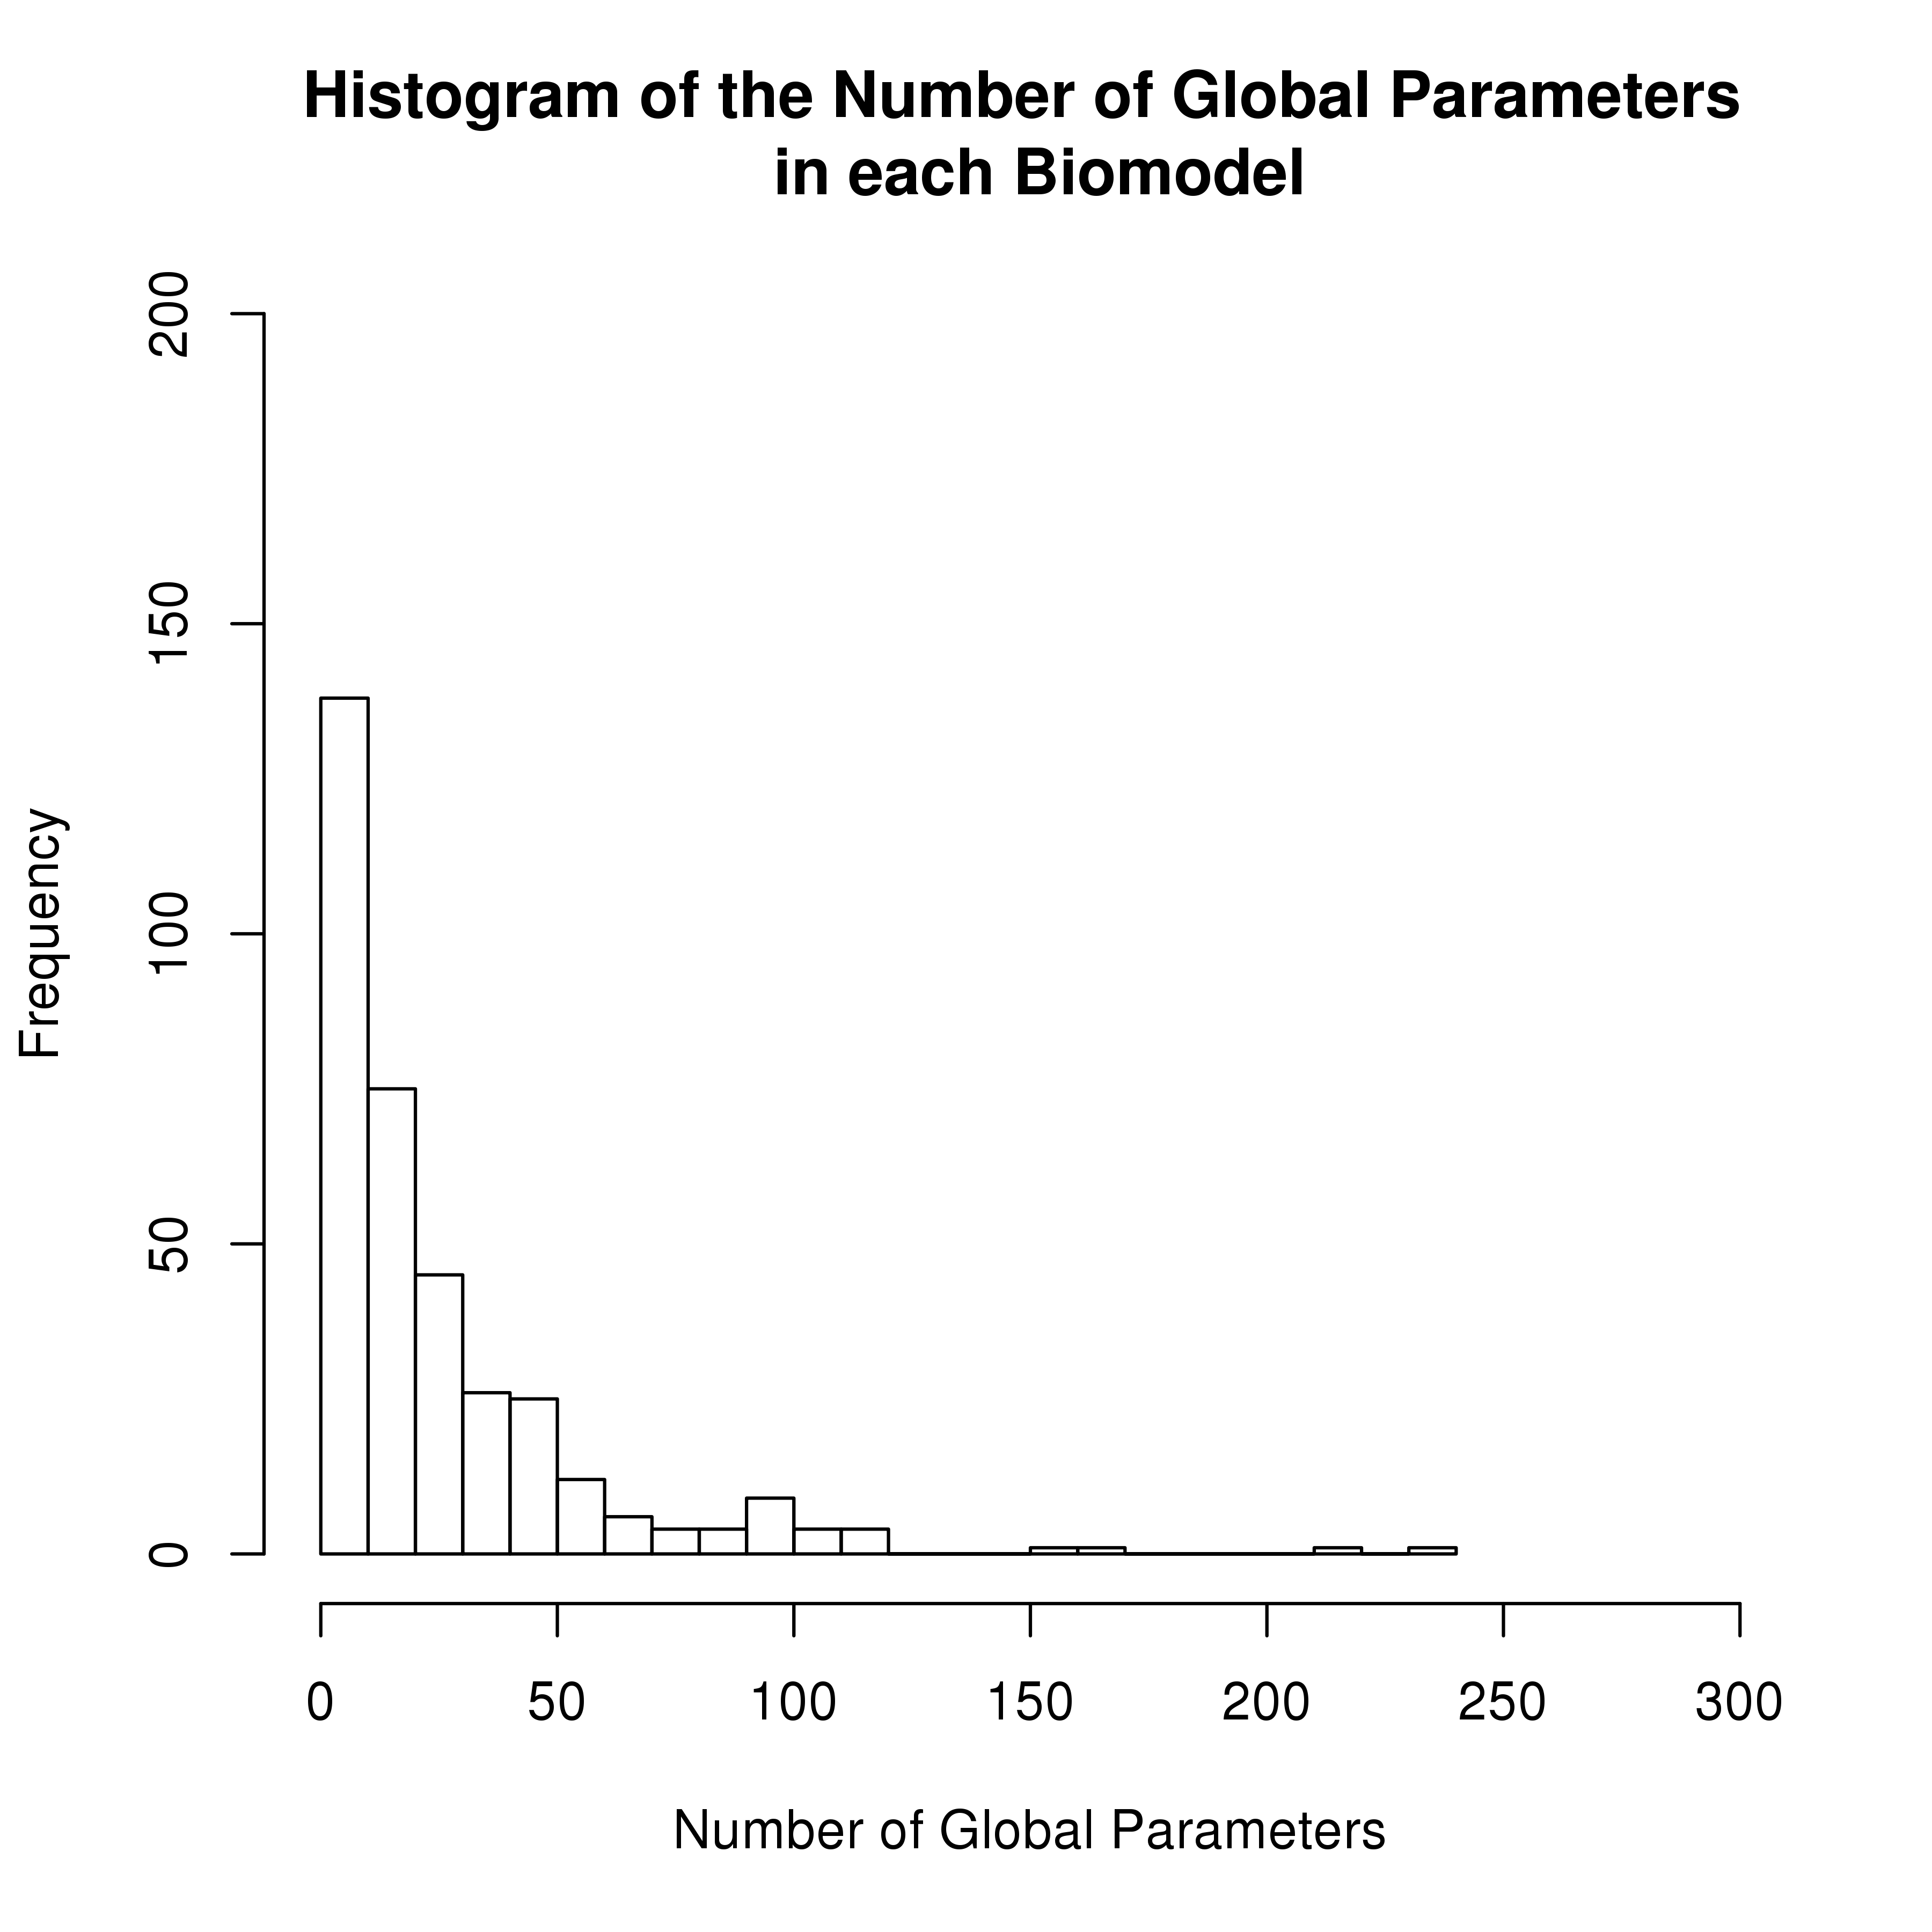
\includegraphics[trim= 1.5mm 5mm 5mm 5mm, clip, scale=0.4]{Poster-images/GlobalParametersHistogram.png}
  The graph above shows the number of global parameters in each biomodel. The majority of models have less than 20 global parameters, with nearly 100 having less than 10 global parameters. This suggests that the models tend to have a low number of global parameters.

 
 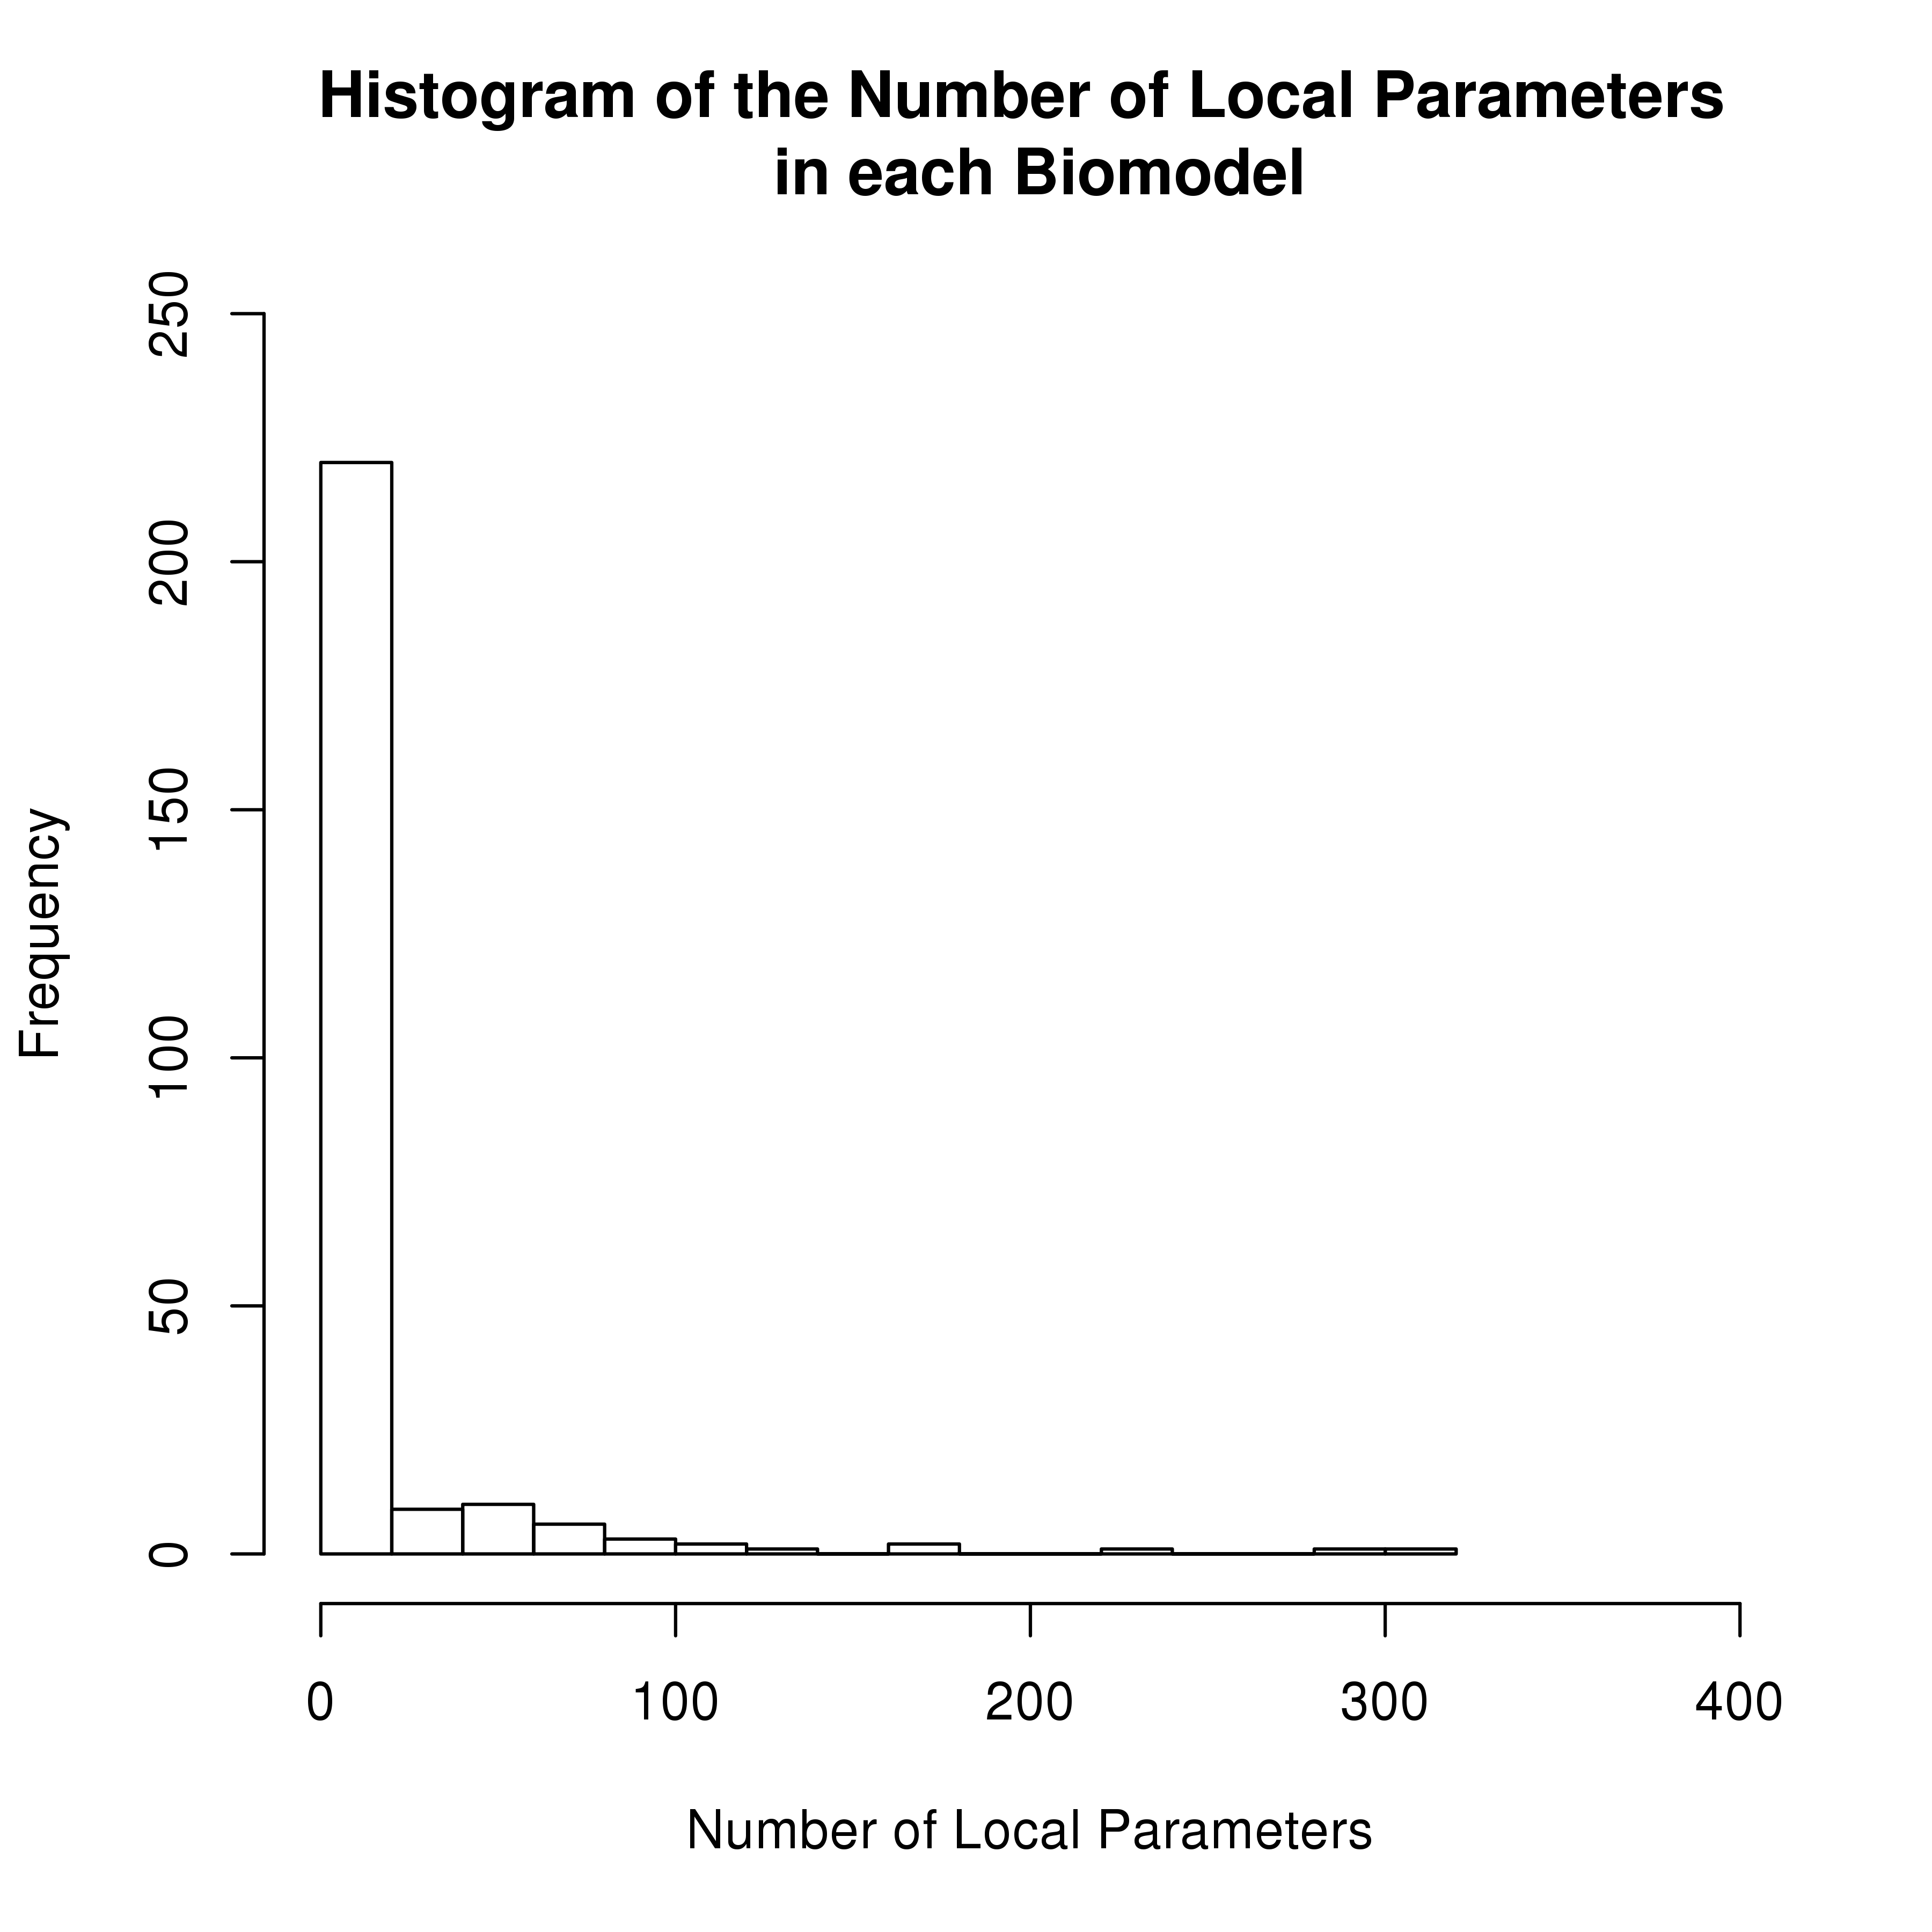
\includegraphics[trim= 1.5mm 5mm 5mm 5mm, clip, scale=0.4]{Poster-images/LocalParametersHistogram.png} 
 The graph above shows the number of local parameters in each biomodel. The vast majority of models have 10 or less local parameters, due to a large proportion 0f models having zero local parameters, since those models are define all their parameters as global parameters. This suggests that the models tend to have a low number of local parameters.
 \end{multicols}
 }
 
\end{poster}

\end{document}